\documentclass{beamer}
\usetheme{CambridgeUS}

\usepackage{tikz}
\usepackage{xeCJK}
\usepackage{amsmath}
\usepackage[version=4]{mhchem}
\usetikzlibrary{graphs}
\usepackage{chemarr}
\usetikzlibrary{automata, arrows, positioning, calc}
\usepackage{fontspec}
\usepackage{caption}
\usepackage{subfigure}
\usepackage{graphicx}

\newcommand{\diag}{\mathrm{diag}}
\newcommand{\tr}{\mathrm{tr}}
\newcommand{\re}{\mathrm{Re}}
\newcommand{\one}{\mathbbm{1}}
\newcommand{\Pnum}{\mathbb{P}}
\newcommand{\Enum}{\mathbb{E}}
\newcommand{\Rnum}{\mathbb{R}}
\newcommand{\dnum}{\mathrm{d}}
\newcommand{\hyper}{{}_2F_1}
\newcommand{\confl}{{}_1F_1}

% 英文字体配置部分
\setmainfont{Source Serif Pro}%Times New Roman
\setsansfont{Source Sans Pro}
\setmonofont{Source Code Pro}
% 中文字体配置部分
\usepackage{xeCJK}%中文字体
\setCJKmainfont{宋体}%正文字体
\setCJKsansfont{黑体}%无衬线字体
\setCJKmonofont{楷体}%等宽字体
\setCJKfamilyfont{boldsong}{Source Han Serif SC Heavy}

\title[单环马氏链环流的大偏差与涨落定理]{单环马氏链环流的大偏差与涨落定理} 
\author{姜瑜浩}

\institute[CSRC]
{\normalsize 指导老师:贾晨 教授\\
% \medskip
北京计算科学研究中心
% \textit{yuhaojiang@csrc.ac.cn}
} 


\begin{document}
\frame{\titlepage}
\begin{frame}{生化反应}
	常见的生化反应模型:
	\captionsetup[figure]{labelfont={bf},name={},labelsep=period}
	\begin{figure}[h]
		\begin{minipage}[t]{0.4\linewidth}
			\centering
			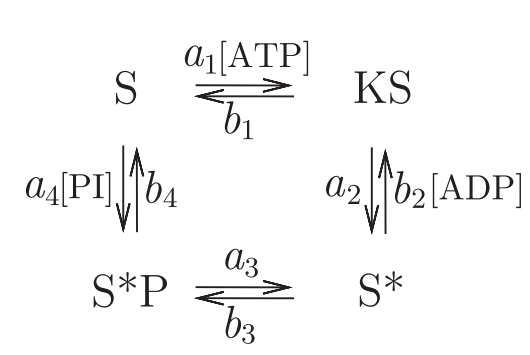
\includegraphics[scale=0.4]{chart/phosphorylation_dephosphorylation_cycle.png}
			\caption{磷酸-脱磷酸化循环}
		\end{minipage}
		\begin{minipage}[t]{0.4\linewidth}
			\centering
			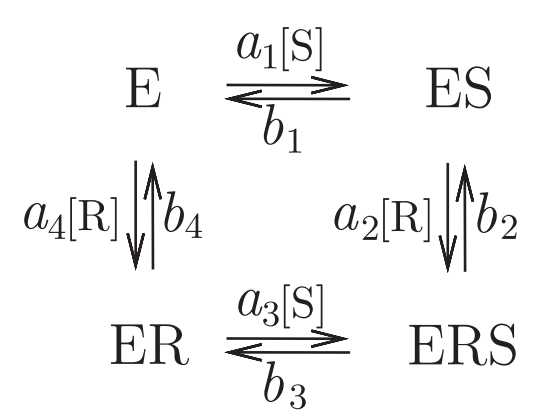
\includegraphics[scale=0.4]{chart/general_modifier_machanism.png}
			\caption{广义的修正机制}
		\end{minipage}
		%\caption{四状态生化反应模型}
	\end{figure}

	\begin{figure}[h]
		\begin{minipage}[t]{0.4\linewidth}
			\centering
			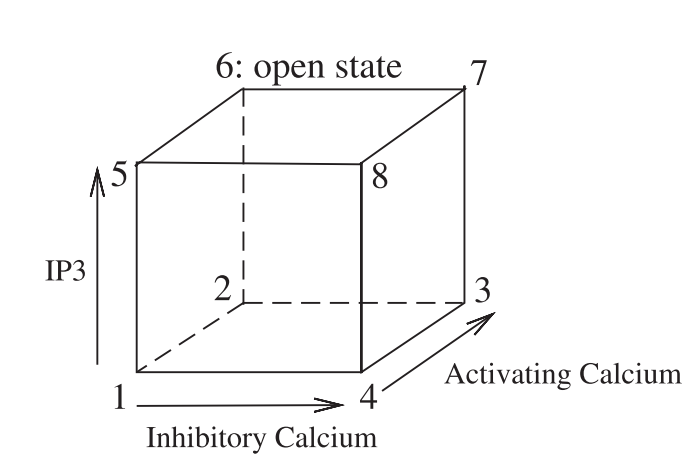
\includegraphics[scale=0.4]{chart/De-Young-Keizer-model.png}
			\caption{De Young-Keizer 模型}
		\end{minipage}
		\begin{minipage}[t]{0.4\linewidth}
			\centering
			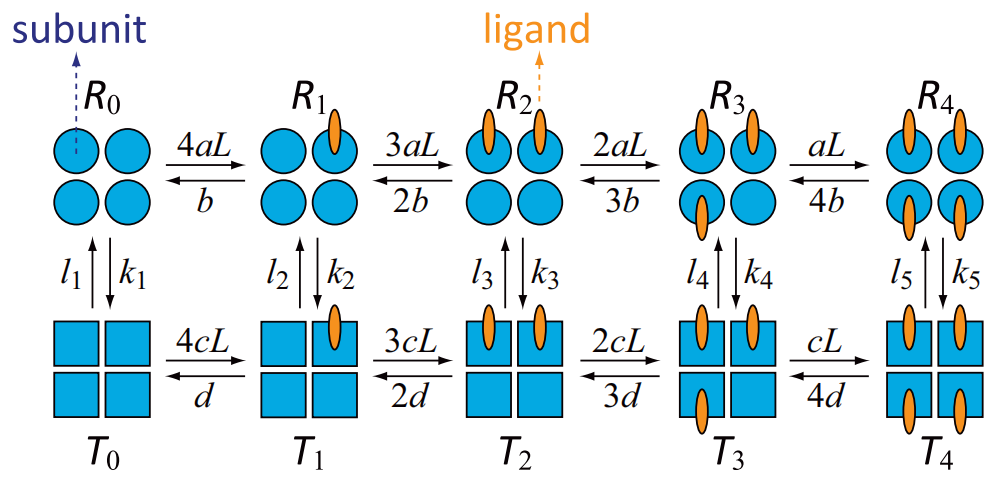
\includegraphics[scale=0.4]{chart/MWC.png}
			\caption{MW模型}
		\end{minipage}
		%\caption{八状态生化反应模型}
	\end{figure}
\end{frame}

\begin{frame} {酶:生物系统中化学反应的催化剂}
	三步 Michaelis-Menten 酶动力学模型:
	$$
		E + S \xrightleftharpoons[k_{-1}]{k_1}
		ES \xrightleftharpoons[k_{-2}]{k_2}
		EP \xrightleftharpoons[k_{-3}]{k_3}
		E + P
	$$
	\begin{figure}[h]
		\centering
		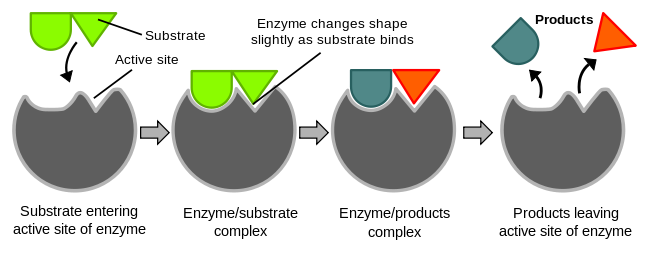
\includegraphics[scale=0.4]{chart/enzyme.png}
	\end{figure}
\end{frame}

\begin{frame}{酶:生物系统中化学反应的催化剂}
	酶化反应的马氏链模型
	\begin{figure}[h]
		\centering
		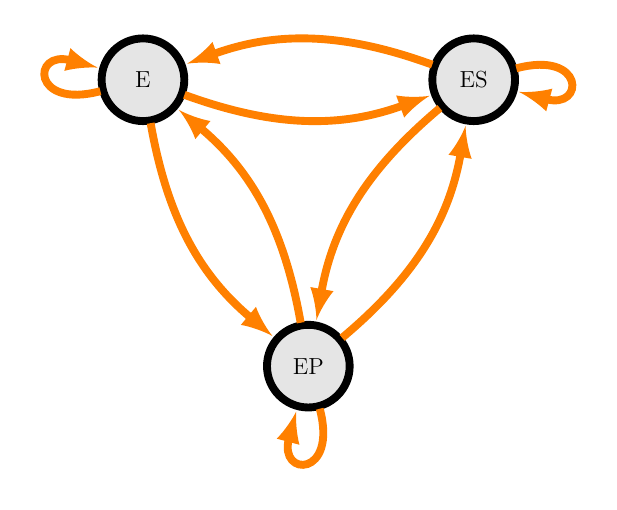
\begin{tikzpicture}[scale=0.7, font=\sffamily]
			\tikzstyle{every node} = [font=\large,scale=0.7]
			% Setup the style for the states
			\tikzset{node style/.style={state,
						minimum width=1.5cm,
						line width=1mm,
						fill=gray!20!white}}
			% Draw the states
			\node[node style] at (0, 0)     (e)     {E};
			\node[node style] at (6, 0)     (es)     {ES};
			\node[node style] at (3, -5.196) (ep) {EP};

			% Connect the states with arrows
			\draw[every loop,
				auto=right,
				line width=1mm,
				>=latex,
				draw=orange,
				fill=orange]
			(e)     edge[bend right=20]             (ep)
			(e)     edge[bend right=20, auto=left]  (es)
			(es)     edge[bend right=20]             (e)
			(es)     edge[bend right=20, auto=left]  (ep)
			(ep) edge[bend right=20]             (es)
			(ep) edge[bend right=20, auto=left]  (e)
			(e) edge[loop left] (e)
			(es) edge[loop right] (es)
			(ep) edge[loop below] (ep);
		\end{tikzpicture}
	\end{figure}
\end{frame}

% \begin{frame}{马氏链中的环流}
% 	\begin{block}{为什么研究上述马氏链中的环?}
% 		考虑上述马氏链中,若环 $E \rightarrow EP \rightarrow ES \rightarrow E$ 出现的频率大于环 $E \rightarrow ES \rightarrow EP \rightarrow E$ 出现的频率,则化学反应整体向正反应进行,否则向负反应进行。
% 		通过研究马氏链中每个环出现的频率,可以研究化学反应整体方向以及反应进程。
% 	\end{block}
% \end{frame}

\begin{frame}{马氏链中的环流}{环擦除方式形成的环}
	\begin{block}{回路的定义}
		马氏链的轨迹中,一段路径的起点和终点相同的,且路径中其他状态各不相同,我们称它为回路,如:$i_1 \to i_2 \to\cdots\to i_s \to i_1$
	\end{block}
	\begin{block}{回路的等价关系}
		记$j_1 \to j_2 \to\cdots\to j_r \to j_1$为另一个回路,若存在一个整数$k$且$r=s$,使得$j_1 = i_{k+1},j_2 = i_{k+2},\cdots,j_n = i_{k+s}$ 成立,则称两个回路等价,其中指标$k+1,k+2,\cdots,k+s$为模$n$后的结果。
	\end{block}
\end{frame}

\begin{frame}{马氏链中的环流}{环擦除方式形成的环}
	\begin{block}{LE环的定义}
		依据回路的等价关系,可以定义等价类,我们称这个等价类为环,并且称所有环构成的集合为环空间 $\mathcal{C}$。例如,回路 $i_1 \to i_2 \to\cdots\to i_s \to i_1$ 所属的环为 $c = (i_1,i_2,\cdots,i_s) \in \mathcal{C}$。
	\end{block}

	\begin{block}{LE(环擦除)环的形成过程}
		\begin{table}[htb!]
			\renewcommand \arraystretch{1} \centering
			\resizebox{\textwidth}{10mm}{
				\begin{tabular}{cccccccccc|p{1em}} \hline\hline
					$n$             & 0       & 1         & 2           & 3           & 4         & 5           & 6             & 7         & 8         \\ \hline
					$\xi_n$         & 1       & 2         & 3           & 3           & 2         & 3           & 4             & 1         & 4         \\ \hline
					$\tilde{\xi}_n$ & {[}1{]} & {[}1,2{]} & {[}1,2,3{]} & {[}1,2,3{]} & {[}1,2{]} & {[}1,2,3{]} & {[}1,2,3,4{]} & {[}1{]}   & {[}1,4{]} \\ \hline
					\text{形成的环} &         &           &             & (3)         & (2,3)     &             &               & (1,2,3,4) &           \\ \hline\hline
				\end{tabular}}
			\caption{导出链的变化过程和轨道中形成的环}\label{trajectory}
		\end{table}
	\end{block}
\end{frame}


\begin{frame}{马氏链中的环流}{生成树方式形成的环}
	\begin{block}{生成树定义}
		记$T$为转移图$G$的有向子图,即$T$的所有边也是$G$的边,$\bar{T}$表示与$T$对应的无向图。满足下列三个条件的$T$被称为图$G$的生成树(极大树):
		\begin{itemize}
			\item $T$是$G$的覆盖子图,即$T$包含$G$的所有顶点。
			\item $\bar{T}$是连通的。
			\item $\bar{T}$没有回路,其中无向图的回路是顶点到自身的无向路径。
		\end{itemize}
	\end{block}
	\begin{block}{ST(生成树)环}
		一般称有向边$l \notin T$为$T$的弦。记$|E|=M$,$|T|= N-1$(T边的数量),那么任意生成树$T$都有$M-N+1$个弦。由于$\bar{T}$是连通的且没有回路,如果添加一根弦$l$到$T$,会导致无向子图$\overline{T \cup \{l\}}$恰好有一条回路。因此$c_l$是由此产生的环,并且和$l$保持同样的指向。由弦生成的环的集合$\mathcal{L} = \{c_l: l\in E\setminus T\}$被称为基本集。
	\end{block}
\end{frame}

\begin{frame}{马氏链中的环流}
	\begin{block}{两种类型环的比较}
		\begin{figure}[h]
			\centering
			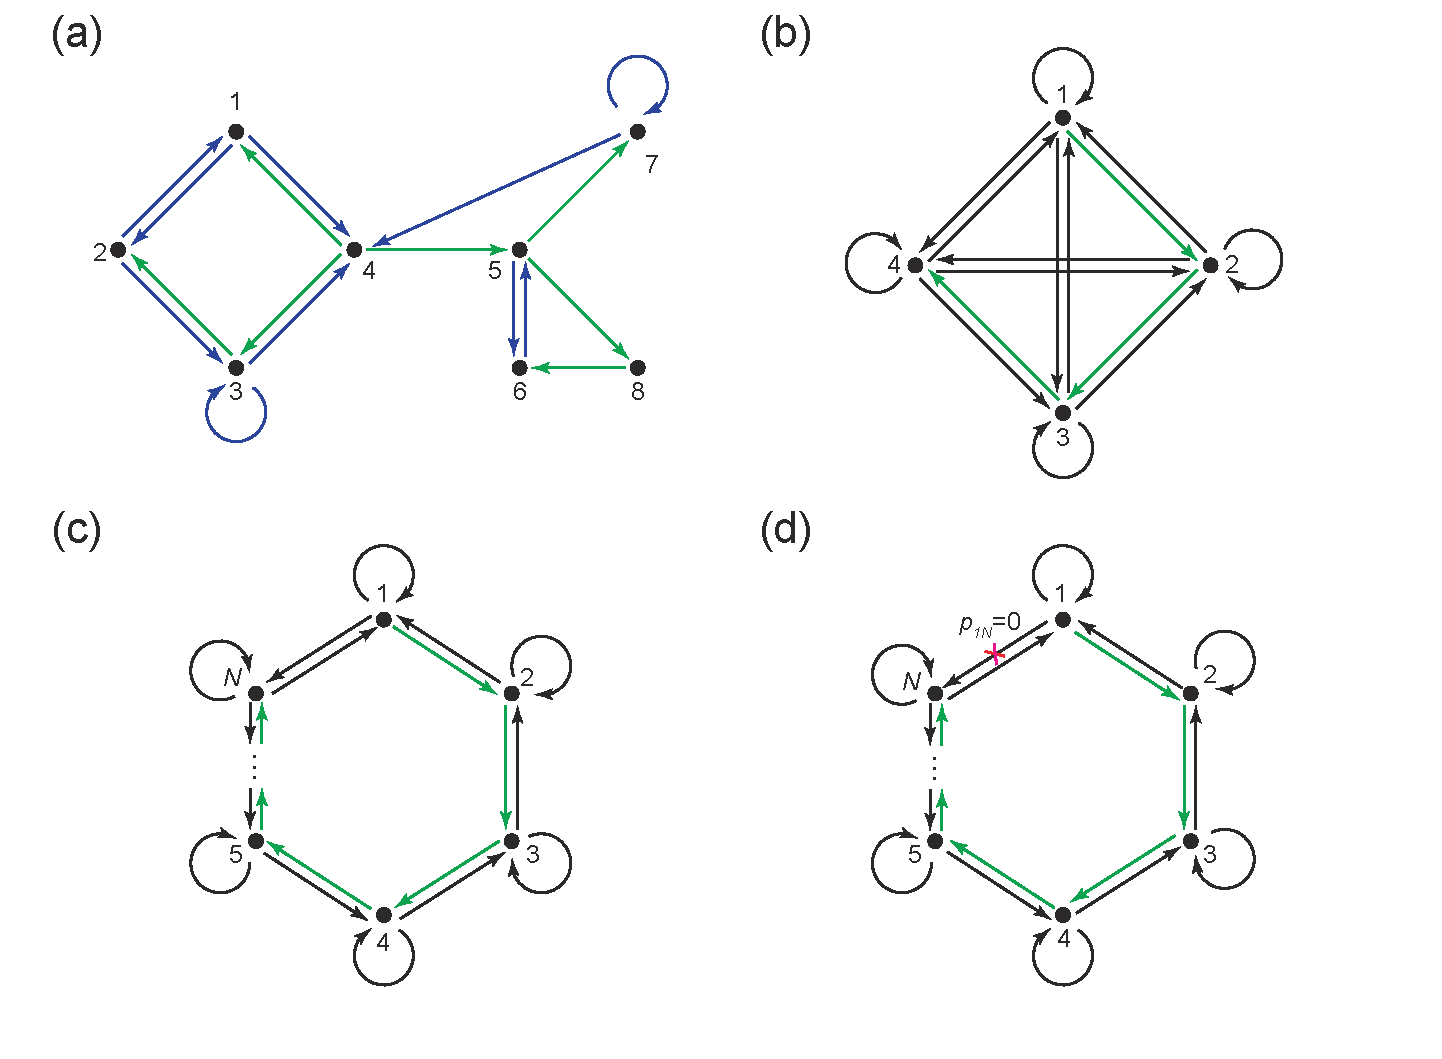
\includegraphics[scale=0.3]{chart/transitiongraph.pdf}
			\caption{{\tiny 马氏链的转移图和相应的生成树 (a) 一般转移图的马氏链, 绿色线表示根节点为4的生成树$T$,并且蓝色线表示$T$的弦 (b) 四状态全连接马氏链,其中每个状态可以转移到自己和其他状态 (c) $N$状态单环马氏链。系统有一个环拓扑。每个状态转移到自身和它两个相邻节点 (d) 一个N状态的单环马尔科夫链,该系统无法从状态$1$转移到状态$N$ (b)-(d)中,绿色箭头表示生成树T}}
			\label{figure:transitiongraph}
		\end{figure}
	\end{block}
\end{frame}

\begin{frame}{马氏链中的环流}{两种定义方式下的环流}
	\begin{block}{LE环流}
		记$N^c_n$ 为环 $c$ 在时刻 $n$ 时总共形成的次数,环 $c$ 在 $n$ 时刻的经验环流为:
		\begin{align*}
			J_n^c & = \frac{1}{n}N^c_n
			%\\ \tilde{J}^c_n &= J^c_n-J^{c-}_n
		\end{align*}
	\end{block}
	\begin{block}{ST环流}
		记$Q^{c_l}_n$表示单位时间通过弦 $l$ 的次数,ST弦和弦是一一对应关系,因此可以用通过弦 $l$ 的次数定义 $c_l$ 形成的次数。 $c_l$ 在 $n$ 时刻的经验环流为:
		\begin{align*}
			Q^{c_l}_n & = \frac{1}{n}\sum_{i=1}^n1_{\{\langle\xi_{i-1},\xi_i\rangle=l\}}
			% \\ \tilde{Q}^{c_l}_n &= Q^{c_l}_n-Q^{c_l-}_n.
		\end{align*}
	\end{block}
\end{frame}

\begin{frame}{大偏差理论}
	\begin{block}{大数定律}
		设独立同分布的随机变量序列 $\left(\mathit{X}_i \right)_{i\in \mathbb{N}}$ 定义于状态空间 $\Gamma=\{1, \cdots, r\}$,概率分布为 $\rho=(\rho_s)_{s \in \Gamma}$。定义 $\rho$ 所处的空间为:
		$$
			\mathfrak{M}_1(\Gamma) = \{\nu = (\nu_1, \nu_2, \cdots, \nu_r)\in [0,1]^r:\sum_{s=1}^r \nu_s = 1\}
		$$
		令经验测度$\mathit{L}_n = \frac{1}{n}\sum_{i=1}^{n}\delta_{\mathit{X}_i} $, 即 $\mathit{L}_n \in \mathfrak{M}_1(\Gamma)$,
		则根据大数定律,有
		\begin{figure}
			\centering
			\ce{$d(\mathit{L}_n, \rho)$ ->[$n\rightarrow \infty$] 0 $\quad$
			$\mathbb{P} - a.s.$}
		\end{figure}
		其中上述度量为全变差距离
		$$
			d(\mu, \nu) = \frac{1}{2} \sum_{s=1}^r |\mu_s - \nu_s|, \quad \mu, \nu \in \mathfrak{M}_1(\Gamma)
		$$
	\end{block}
\end{frame}

\begin{frame}{大偏差理论}
	\begin{block}{Level-1 大偏差 (Cramers 定理)}
		$(\mathit{X}_i)_{i\in \mathbb{N}}$是上述定义的独立同分布的随机变量序列,相应的经验测度为 $\mathit{L}_n = \frac{1}{n} \sum_{i=1}^n \delta_{\mathit{X}_i}$。那么,对于 $\forall a>0$,有:
		$$
			\lim_{n \rightarrow \infty} \frac{1}{n} \log \mathbb{P} \left(\mathit{L}_n \in \mathit{B}_a^c(\rho)\right) = -\inf_{\nu \in \mathit{B}_a^c(\rho)} \mathit{I}(x)
		$$
		其中 $\mathit{B}_a(\rho)=\{\nu \in \mathfrak{M}_1(\Gamma): d(\nu,  \rho) \le a\}$ 是 $\rho$ 的邻域,$\mathit{B}_a^c(\rho) = \mathfrak{M}_1(\Gamma) \backslash  \mathit{B}_a(\rho)$,且称
		$$
			\mathit{I}_{\rho}(\nu) = \sum_{s=1}^r \nu_s \log \left(\frac{\nu_s}{\rho_s}\right)
		$$
		为速率函数。
	\end{block}
\end{frame}

\begin{frame}{大偏差理论}
	\begin{block}{Level-2 大偏差 (Sanov定理)}
		在随机变量序列 $(\mathit{X}_i)_{i\in \mathbb{N}}$ 上,定义对经验测度
		$\mathit{L}_n^2 = \frac{1}{n} \sum_{i=1}^n \delta_{(\mathit{X}_i, \mathit{X}_{i+1})}$

		不妨令 $\mathit{X}_{n+1} = \mathit{X}_1$(当$n\rightarrow \infty$时,该假设对$\mathit{L}_n^2$ 取值无影响。)
		则 $\mathit{L}_n^2$ 所在的概率测度空间
		$\widetilde{\mathfrak{M}}_1(\Gamma \times \Gamma) = \{\nu=(\nu_{st}) \in \mathfrak{M}_1(\Gamma \times \Gamma):$ \\$ \sum_{t} \nu_{st} = \sum_{t} \nu_{ts}, \forall s\}.$

			Sanov 证明了对于 $\forall a > 0$,有:
		$$
			\lim_{n \rightarrow \infty} \frac{1}{n} \log \mathbb{P}(\mathit{L}_n^2 \in B_a^c(\rho \times \rho))
			= - \inf_{\nu \in B_a^c(\rho \times \rho)} \mathit{I}_{\rho}^2(\nu)
		$$
		其中 $B_a(\rho \times \rho) = \{\nu \in \widetilde{\mathfrak{M}}_1(\Gamma \times \Gamma): d(\nu, \rho \times \rho) \le a\}$,$\bar{\nu}_s = \sum_t \nu_{st}$,且速率函数为
		$$
			\mathit{I}_{\rho}^2(\nu) = \sum_{s,t} \nu_{st} \log\left(\frac{\nu_{st}}{\bar{\nu_s}\rho_t}\right)
		$$
	\end{block}
\end{frame}

\begin{frame}{环流的大偏差原理}
	\begin{block}{环流大偏差原理的定义}
		若满足下列三个条件,则称经验LE环流 $(J_n^c)_{c \in \mathcal{C}}$ 为满足速率函数为 $I_J:\mathcal{V}\rightarrow [0,\infty]$ 的大偏差原理:
		\begin{itemize}
			\item 对于$\forall \alpha \geqslant 0$,水平集$\{x \in \mathcal{V}: I_{J}(x) \leqslant \alpha\}$是紧的。
			\item 对于任意开集$U \subset \mathcal{V}$,
			      \begin{equation}\label{def1}
				      \varliminf_{n\to\infty}\frac{1}{n}\log\mathbb{P}((J^c_n)_{c\in\mathcal{C}}\in U)\ge-\inf_{x\in U}I_J(x).
			      \end{equation}
			\item 对于任意闭集$F \subset \mathcal{V}$,
			      \begin{equation}\label{def2}
				      \varlimsup_{n\to \infty}\frac{1}{n}\log\mathbb{P}((J^c_n)_{c\in\mathcal{C}}\in F)\le -\inf_{x\in F}I_J(x).
			      \end{equation}
		\end{itemize}
	\end{block}
\end{frame}

\begin{frame}{环流的大偏差原理}
	\begin{block}{环流大偏差速率函数}
		定义中的条件$(ii)$和$(iii)$表明,对任意 $(\nu^c)_{c\in\mathcal{C}}\in\mathcal{V}$,速率函数满足:
		\begin{equation*}\label{LDP}
			\mathbb{P}(J^c_n=\nu^c,\;\forall c\in\mathcal{C})\propto e^{-n I_J(\nu)},\;\;\;n\to\infty,
		\end{equation*}

		假设轨道满足周期边界条件,还可得LE经验环流的联合分布为:
		\begin{equation*}\label{joint}
			\begin{split}
				\mathbb{P}\left(J^c_n=\nu^c,\;\forall c\in\mathcal{C}\right)
				=&\;\mathbb{P}\left(N^c_n=k^c,\;\forall c\in\mathcal{C}\right)\\
				=&\;|G_n(k)|\prod_{c\in\mathcal{C}}\left(\gamma^c\right)^{k^c},
			\end{split}
		\end{equation*}
		其中$\nu^c = k^c/n$,$G_n(k)$表示$n$时刻可能形成的轨道的集合,$\gamma^c = p_{i_1i_2}p_{i_2i_3}\cdots p_{i_si_1}$表示沿该环所有转移概率的乘积。并且称该类轨道为容许轨道。
	\end{block}
\end{frame}

\begin{frame}{环流的大偏差原理}{环流大偏差速率函数}
	例:三状态马氏链的一段轨道中,环的数量$k=(k^c)_{c\subset \mathcal{C}}$为:
	\begin{equation*} \label{trajectory_ex}
		k^3 = k^{12} = k^{23} = k^- = 1, ~~~ k^1 = k^2 = k^{13} = k^+= 0
	\end{equation*}
	那么在时刻$n=8$,有8个容许轨道,如表\ref{table:all possible trajectories}所示。

	\begin{table}[htb!]
		\renewcommand\arraystretch{0.8}
		\begin{tabular}{cccccccccc}
			\hline
			$m$     & 0 & 1 & 2 & 3 & 4 & 5 & 6 & 7 & 8 \\\hline
			$\xi_m$ & 1 & 3 & 3 & 2 & 3 & 2 & 1 & 2 & 1 \\\hline
			$\xi_m$ & 1 & 3 & 2 & 3 & 3 & 2 & 1 & 2 & 1 \\\hline
			$\xi_m$ & 1 & 3 & 3 & 2 & 1 & 2 & 3 & 2 & 1 \\\hline
			$\xi_m$ & 1 & 3 & 2 & 1 & 2 & 3 & 3 & 2 & 1 \\\hline
			$\xi_m$ & 1 & 2 & 3 & 3 & 2 & 1 & 3 & 2 & 1 \\\hline
			$\xi_m$ & 1 & 2 & 3 & 2 & 1 & 3 & 3 & 2 & 1 \\\hline
			$\xi_m$ & 1 & 2 & 1 & 3 & 3 & 2 & 3 & 2 & 1 \\\hline
			$\xi_m$ & 1 & 2 & 1 & 3 & 2 & 3 & 3 & 2 & 1 \\\hline
		\end{tabular}\centering
		\caption{三状态马氏链中,8个容许轨道,环$(3), (12), (23)$和$(1,3,2)$形成一次,环$(1), (2), (13)$和$(1,2,3)$没有形成过}
		\label{table:all possible trajectories}
	\end{table}
\end{frame}

\begin{frame}{环流的大偏差原理}{环流大偏差速率函数}
	\begin{figure}[htb!]
		\centering
		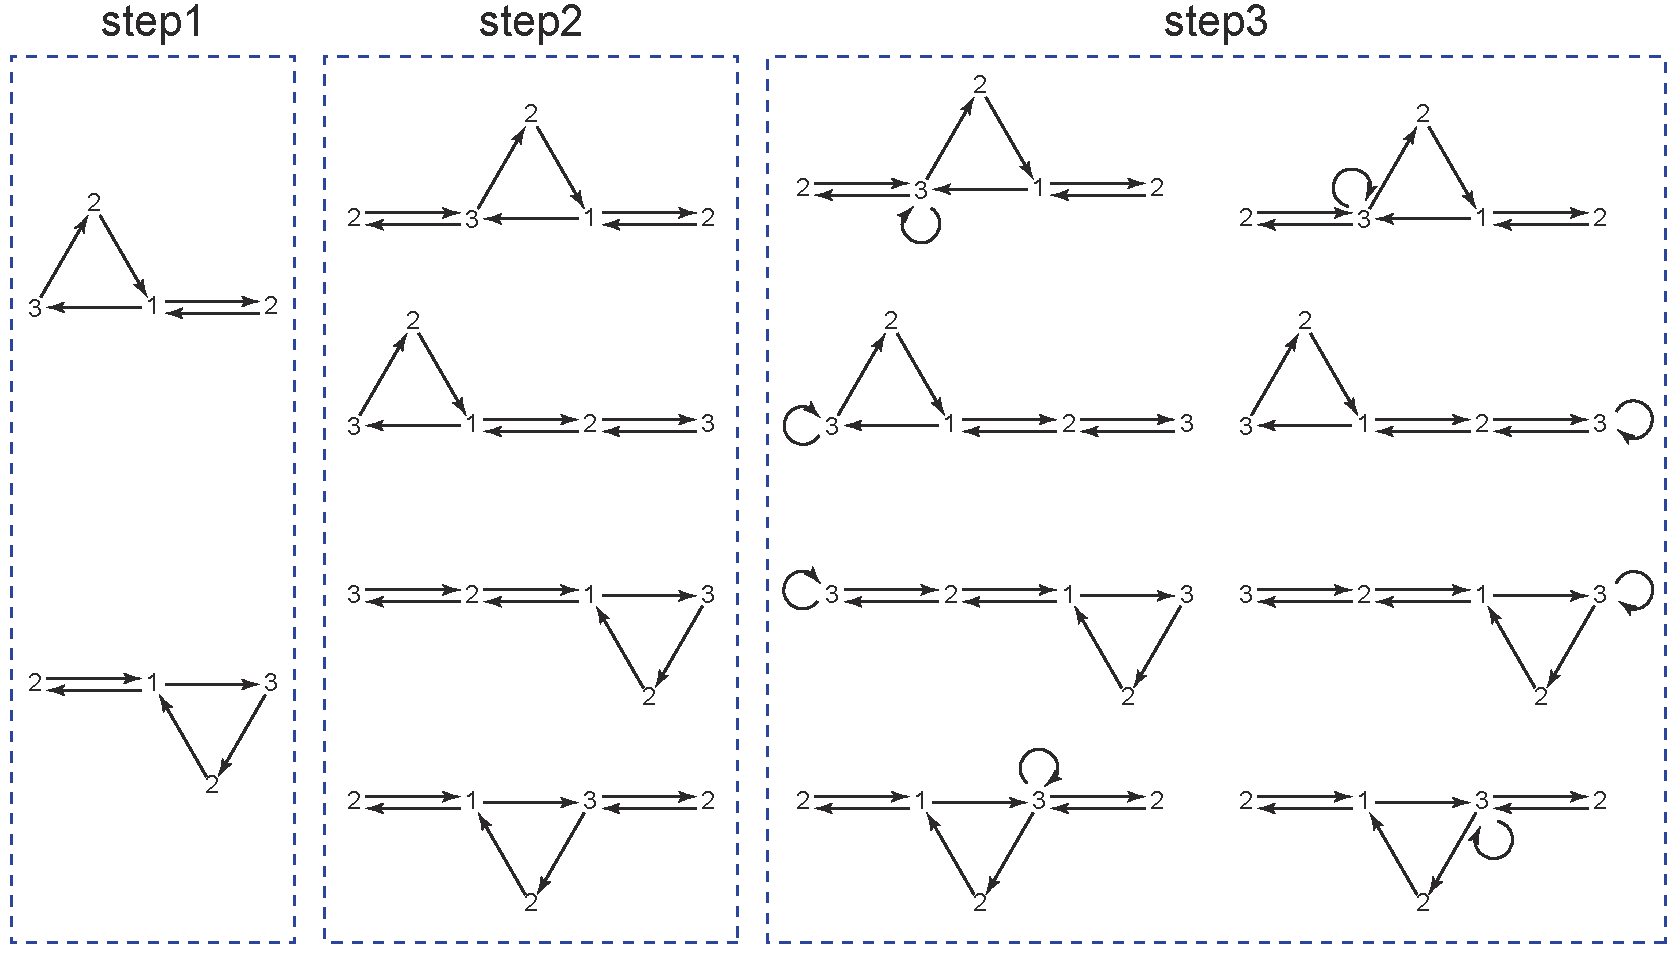
\includegraphics[scale=0.35]{chart/insertiongraph.pdf}
		\caption{{\tiny 构建所有容允许轨道的环插入法示意图。依然使用\ref{trajectory_ex}中的例子。环插入法分为三步:首先我们将所有包含初始状态的环插入轨道,接下来我们将所有剩余的两元环插入轨道,最后我们将所有剩余的一元环插入轨道。经过这三步的环插入,找到了所有八个容许轨道。}}
		\label{figure:insertion}
	\end{figure}
\end{frame}

\begin{frame}{环流的大偏差原理}{环流大偏差速率函数}
	\begin{block}{计算容许轨道空间的规模}
		依据图中所示的计算方法,对于所有单环马氏链,可得容许轨道空间的规模为:
		$$|G_n(k)|=A_1A_2A_3 $$
		其中:{\footnotesize
		\begin{equation*}\label{formula:A1}
			A_1 = \binom{k^1+k^{12}+k^{1N}+k^{+}+k^{-}}{k^1,k^{12},k^{1N},k^{+},k^{-}}
			:= \frac{(k^1+k^{12}+k^{1N}+k^{+}+k^{-})!}{k^1!\;k^{12}!\;k^{1N}!\;k^{+}!\;k^{-}!},
		\end{equation*}
		\begin{equation*}
			A_2 = \sum_{l^{2}+m^{2}=k^{23}}\dots\sum_{l^{N-1}+m^{N-1}=k^{N-1,N}}
			\prod_{i=2}^{N-1}\binom{l^{i}+l^{i-1}+k^{+}-1}{l^{i}}\prod_{i=2}^{N-1}\binom{m^{i}+m^{i+1}+k^{-}-1}{m^{i}},
		\end{equation*}
		\begin{equation*}\label{formula:A3}
			A_3 = \prod_{i=2}^N\binom{\sum_{c\ni i}k^{c}-1}{k^{i}}.
		\end{equation*}}
	\end{block}
\end{frame}

\begin{frame}{环流的大偏差原理}{环流大偏差速率函数}
	环流大偏差速率函数表达式:
	\begin{equation*}
		\begin{split}
			I_J(\nu) &= -\lim_{n\to\infty}\frac{1}{n}\log\mathbb{P}\left(J^c_n=\nu^c,\;\forall c\in\mathcal{C}\right)\\
			&= -\lim_{n\to\infty}\frac{1}{n}\left[\log A_1+\log A_2+\log A_3+\sum_{c\in\mathcal{C}}k^c\log\gamma^c\right].
		\end{split}
	\end{equation*}
	化简可得:
	\begin{equation*}\label{ratefunction}
		\begin{split}
			I_J(\nu) =&\; \left[h\left(\nu^{12}\right)+h\left(\nu^{1N}\right)
				+h\left(\nu^+\right)+h\left(\nu^-\right)-h\left(\nu^{12}+\nu^{1N}+\nu^++\nu^-\right)\right] \\
			&\;+\inf_{X\in V(\nu)}F_{\nu}(X)+\sum_{i\in S}\left[ h\left(\nu_i-\nu^i\right)+h\left(\nu^i\right)
				-h\left(\nu_i\right)\right]-\sum_{c\in\mathcal{C}}\nu^c\log\gamma^c,
		\end{split}
	\end{equation*}
	其中$h(x) = x \log x$,$\nu^c = \frac{k^c}{n}, \nu_i=\sum_{c\ni i}\nu^c$。
\end{frame}

\begin{frame}{环流的大偏差原理}{环流大偏差速率函数}
	由环流大偏差速率函数表达式:
	\begin{equation*}
		\begin{split}
			I_J(\nu) &= -\lim_{n\to\infty}\frac{1}{n}\log\mathbb{P}\left(J^c_n=\nu^c,\;\forall c\in\mathcal{C}\right)\\
			&= -\lim_{n\to\infty}\frac{1}{n}\left[\log A_1+\log A_2+\log A_3+\sum_{c\in\mathcal{C}}k^c\log\gamma^c\right].
		\end{split}
	\end{equation*}
	证明环流大偏差速率函的存在唯一性,转换为优化问题:
	\begin{equation*}
		\inf_{X\in V(\nu)}F_{\nu}(X) = F_{\nu}(x^i,y^i),
	\end{equation*}
	的存在唯一性。
\end{frame}

\begin{frame}{环流的大偏差原理}{环流大偏差速率函数}
	定义相应的拉格朗日函数:
	\begin{align*}
		\mathcal{A}_{\nu}(X,\lambda) = F_{\nu}(X) + \sum_{i=2}^{N-1} \lambda_i \left(x^{i} + y^{i} - \nu^{i,i+1}\right), \;\;\;\forall \nu\in\mathcal{V}
	\end{align*}
	其中 $X=(x^i,y^i)_{2\le i\le N-1}\in V(\nu)$ 并且 $\lambda=(\lambda_i)_{2\le i\le N-1}\in \mathbb{R}^{N-2}$ \\
	经过化简得到:
	\begin{equation}\label{equations}
		\begin{split}
			\frac{x^{i}}{x^{i-1}+x^{i}+\nu^+}
			\,\frac{x^{i}+\nu^+}{x^{i}+x^{i+1}+\nu^+}
			&= \frac{y^{i}+\nu^-}{y^{i-1}+y^{i}+\nu^-}
			\,\frac{y^{i}}{y^{i}+y^{i+1}+\nu^-}=e^{-\lambda_i},\\
			x^{i} + y^{i} &= \nu^{i,i+1},\qquad 2\le i\le N-1.
		\end{split}
	\end{equation}
	其中 $x^1=\nu^{12}$,$x^N=0$,$y^1=0$ 和 $y^N=\nu^{1N}$。\\
	最终我们证明了该方程 \ref{equations} 的解存在且唯一
\end{frame}

\begin{frame}{环流的大偏差原理}{环流大偏差速率函数}
	环流大偏差速率函数的性质:
	\begin{itemize}
		\item 有界性
		\item 凸函数
		\item 对称性:上述推导中,都是假设马氏链从状态1出发,我们证明了从任意状态出发都可以得到此结果
		\item 连续性:在$[0, +\infty)$ 上连续
	\end{itemize}
\end{frame}

\begin{frame}{环流的大偏差原理}{环流大偏差速率函数}
	\begin{block}{三环马氏链}
		环流大偏差速率函数,可简化为:
		\begin{align*}
			I_J(\nu) & =
			\sum_{i\in S} \left[\nu^{i}\log \left(\frac{\nu^{i}/\nu_i}{J^i/J_i}\right) + (\nu_i - \nu^i)\log \left(\frac{(\nu_i - \nu^i)/\nu_i}{(J_i - J^i)/J_i} \right)
			\right]                                                                                                               \\
			         & + \sum_{c \in \mathcal{C}, |c|\neq 1} \nu^{c} \log \left(\frac{\nu^{c}/\tilde{\nu}}{J^c/\tilde{J}}\right).
		\end{align*}
		\begin{figure}[h]
			\centering
			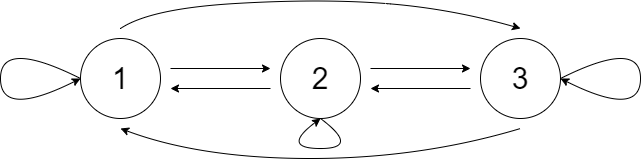
\includegraphics[scale=0.3]{chart/3-state.png}
			\caption*{状态转移图}
		\end{figure}
	\end{block}
\end{frame}

\begin{frame}{环流的大偏差原理}{环流大偏差速率函数}
	\begin{block}{状态 1 到状态 N 的转移概率为 0 的单环马氏链的速率函数}
		环流大偏差速率函数,可简化为:
		{\scriptsize
		\begin{align*}
			I_J(\nu) = \sum_{i\in S}\left[\nu^i\log\left(\frac{\nu^i/\nu_i}{J^i/J_i}\right)
				+\nu^{i,i+1}\log\left(\frac{\nu^{i,i+1}/\nu_i}{J^{i,i+1}/J_i}\right)+\left(\nu^{i-1,i}+\nu^+\right)\log\left(\frac{\left(\nu^{i-1,i}+\nu^+\right)/\nu_i}
				{\left(J^{i-1,i}+J^+\right)/J_i}\right)\right].
		\end{align*}}
		\begin{figure}[h]
			\centering
			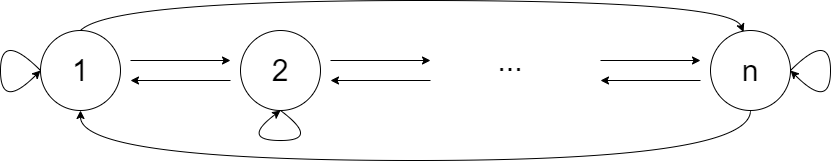
\includegraphics[scale=0.3]{chart/n-state2.png}
			\caption*{状态转移图}
		\end{figure}
	\end{block}
\end{frame}

\begin{frame}{环流的大偏差原理}{环流大偏差速率函数}
	\begin{block}{净环流大偏差速率函数}
		记LE经验净环流为 $(\tilde{J}^{c}_n)_{c\in\mathcal{C}}$,由收缩原理可以得到:
		\begin{align*}
			\mathbb{P}\left(\tilde{J}^{+}_n = x\right)
			 & =\;\mathbb{P}\left(J^{+}_n-J^{-}_n = x\right)                                             \\
			 & =\;\sum_{\nu^{+}-\nu^{-}=x}\mathbb{P}\left(J^{c}_n=\nu^{c},\forall c\in\mathcal{C}\right) \\
			 & \propto\sum_{\nu^{+}-\nu^{-}=x} e^{-nI_J(\nu)}.
		\end{align*}
		因此$\tilde{J}^+_n$满足大偏差原理,相应的速率函数$I_{\tilde{J}}$为:
		\begin{equation*}
			I_{\tilde{J}}(x)=\inf_{\{\nu\in\mathcal{V}:\nu^{+}-\nu^{-}= x\}}I_J(\nu).
		\end{equation*}
	\end{block}
\end{frame}

\begin{frame}{环流的大偏差原理}{一般马氏链的ST环流的大偏差}
	\begin{block}{对经验测度的大偏差}
		定义$n$时刻的对经验测度$R_n:E\rightarrow[0,1]$为
		\begin{equation*}
			R_n(i,j) = \frac{1}{n}\sum_{m=1}^n1_{\{\xi_{m-1}=i,\xi_m=j\}},
		\end{equation*}
		对经验测度满足下面的大偏差原理:
		\begin{equation*}
			\mathbb{P}(R_n(i,j)=R(i,j),\;\forall\langle i,j\rangle\in E)\propto e^{-nI_{\mathrm{pair}}(R)},\;\;\;n\to\infty,
		\end{equation*}
		其中的速率函数为 $I_{\mathrm{pair}}:\mathcal{M}\rightarrow[0,\infty]$为
		\begin{equation*}
			I_{\mathrm{pair}}(R) = \sum_{\langle i,j\rangle\in E}R(i,j)\log\frac{R(i,j)}{R(i)p_{ij}}
		\end{equation*}
		其中$R(i)=\sum_{j\in S}R(i,j)$
	\end{block}
\end{frame}

\begin{frame}{环流的大偏差原理}{一般马氏链的ST环流的大偏差}
	\begin{block}{ST环流大偏差速率函数}
		对经验测度可以被分解为下面ST环流的加权和:
		\begin{equation*}
			R_n(i,j) = \sum_{c_l\in\mathcal{L}}H^{c_l}(i,j)Q^{c_l}_n,
		\end{equation*}
		其中:
		\begin{equation*}\label{cycle function2}
			H^{c_l}(i,j)
			=\left\{\begin{aligned}
				1,  &  &  & \text{if } \langle i,j\rangle \in c_l \text{ and }\langle i,j\rangle \in T, \text{ or } \langle i,j\rangle=l, \\
				-1, &  &  & \text{if } \langle i,j\rangle\notin c_l,\langle j,i\rangle \in c_l,\text{ and }\langle i,j\rangle \in T,      \\
				0,  &  &  & \text{otherwise}.                                                                                             \\
			\end{aligned}\right.
		\end{equation*}
		并且该分解是唯一的。
	\end{block}
\end{frame}

\begin{frame}{环流的大偏差原理}{一般马氏链的ST环流的大偏差}
	\begin{block}{ST环流大偏差速率函数}
		如果$R_n =\sum_{c_l \in \mathcal{L}}\nu^{c_l}H^{c_l}$,那么对任意$c_l \in \mathcal{L}$会有$\nu^{c_l}=Q_n^{c_l}$。由上式分解的唯一性,可得:
		{\footnotesize
		\begin{equation*}
			\mathbb{P}(Q_n^{c_l}=\mu^{c_l},\;\forall c_l\in\mathcal{L})
			=\mathbb{P}\left(R_n(i,j)=\sum_{c_l\in\mathcal{L}}\mu^{c_l}H^{c_l}(i,j),\;\forall\langle i,j\rangle\in E\right)
			\propto e^{-n I_{\mathrm{pair}}\left(\sum_{c_l\in\mathcal{L}}\mu^{c_l}H^{c_l}\right)}.
		\end{equation*}}
		这表明ST经验环流$(Q_n^{c_l})_{c_l\in\mathcal{L}}$满足大偏差原理,相应的速率函数$I_Q:\mathcal{M}\rightarrow[0,\infty]$为:
		\begin{equation*}\label{formula:I_Q}
			I_Q(\mu)=I_{\mathrm{pair}}\left(\sum_{c_l\in\mathcal{L}}\mu^{c_l}H^{c_l}\right).
		\end{equation*}
	\end{block}
\end{frame}

\begin{frame}{环流的涨落定理}{单环马氏链LE环流的涨落定理}
	\begin{block}{强对称关系}
		单环马氏链LE环流满足强对称关系,即:
		\begin{align}
			  & \;k^+ \mathbb{P}\left(N^+_n=k^+,N^-_n=k^- -1,N^c_n=k^c,\;\forall c\neq C^+,C^-\right)                                    \\
			= & \; \left(\frac{\gamma^+}{\gamma^-}\right)\mathbb{P}\left(N^+_n=k^+ -1,N^-_n=k^-,N^c_n=k^c,\;\forall c\neq C^+,C^-\right)
		\end{align}
		该式中 $C^+ = (1,2,\cdots,N)$ 和 $C^- = (1,N,\cdots,2)$ 表示单环系统中两个 N 元环,$N^+_n$ 和 $N^-_n$ 分别表示 n 时刻环  $C^+$ 和 $C^-$ 分别形成的数量。并且 $\gamma^+ = p_{12}p_{23}\cdots p_{N1}$ 和 $\gamma^- = p_{1N}p_{N,N-1}\cdots p_{21}$ 分别是环 $C^+$ 和环 $C^-$中的转移概率的乘积。
	\end{block}
\end{frame}

\begin{frame}{环流的涨落定理}{单环马氏链LE环流的涨落定理}
	LE环流满足的各种涨落定理
	\begin{itemize}
		\item 暂态涨落定理:
		      \begin{equation*}\label{theorem:transient fluatuation}
			      \mathbb{P}\left(N^+_n=k^+,N^-_n=k^-,\cdots\right)
			      = \mathbb{P}\left(N^+_n=k^-,N^-_n=k^+,\cdots\right)\left(\frac{\gamma^+}{\gamma^-}\right)^{k^+-k^-}.
		      \end{equation*}

		\item Kurchan-Lebowitz-Spohn 类型涨落定理:
		      \begin{equation*}
			      g_n(\lambda^+,\lambda^-,\cdots)
			      = g_n\left(\lambda^--\log\frac{\gamma^+}{\gamma^-},
			      \lambda^++\log\frac{\gamma^+}{\gamma^-},\cdots\right), 
				%   ~~~~
				%   g_n(\lambda^+,\lambda^-,\cdots)
				%   = \mathbb{E}\left[e^{\lambda^+N^+_n+\lambda^-N^-_n+\sum_{c\neq C^+,C^-}\lambda^cN^c_n}\right].
		      \end{equation*}

		\item Gallavotti-Cohen 类型涨落定理:
		      \begin{equation*}
			      I_J(\cdots,\nu^+,\nu^-)=I_J(\cdots,\nu^-,\nu^+)-\left(\log\frac{\gamma^+}{\gamma^-}\right)(\nu^+-\nu^-).
		      \end{equation*}
	\end{itemize}
\end{frame}

\begin{frame}{环流的涨落定理}{单环马氏链LE环流的涨落定理}
	LE净环流满足的各种涨落定理
	\begin{itemize}
		\item 暂态涨落定理:
		      \begin{equation*}
			      \frac{\mathbb{P}(\tilde{J}^+_n=x)}{\mathbb{P}(\tilde{J}^+_n=-x)}
			      = \left(\frac{\gamma^+}{\gamma^-}\right)^{nx}.
		      \end{equation*}

		\item Kurchan-Lebowitz-Spohn 类型涨落定理:
		      \begin{equation*}
			      \tilde{g}_n(\lambda)=\tilde{g}_n\left(-\left(\lambda+\log\frac{\gamma^+}{\gamma^-}\right)\right).
		      \end{equation*}
		\item 积分涨落定理 :
		      \begin{equation*}
			      \mathbb{E}\left[e^{\lambda n\tilde{J}^+_n}\right]=1.
		      \end{equation*}

		\item Gallavotti-Cohen 类型涨落定理:
		      \begin{equation*}
			      \tilde{I}_J(x)=\tilde{I}_J(-x)-\left(\log\frac{\gamma^+}{\gamma^-}\right)x.
		      \end{equation*}
	\end{itemize}
\end{frame}

\begin{frame}{环流的涨落定理}{一般马氏链LE环流的涨落定理}
	\begin{block}{相似环}
		记 $c_1=(i_1,i_2,\cdots,i_s)$ 和 $c_2=(j_1,j_2,\cdots,j_r)$ 是两个环。如果 $s=r$ 且 $\{i_1,i_2,\cdots,i_s\}=\{j_1,j_2,\cdots,j_r\}$,则称环 $c_1$ 和环 $c_2$ 相似。因此,下面六个环
		$(1,2,3,4), (1,2,4,3), (1,3,2,4), (1,3,4,2), (1,4,2,3), (1,4,3,2)$
		互为相似关系。
	\end{block}
	\begin{block}{一般马氏链LE经验环流的对称关系}
		一般马氏链,如果环$c_1$和$c_2$相似,LE经验环流 $(J^c_n)_{c\in\mathcal{C}}$,$J_n^c=N_n^c/n$ 满足下列的对称关系:
		\begin{equation*}
			\frac{k^{c_1} \Pnum(N^{c_1}_n=k^{c_1},N^{c_2}_n=k^{c_2}-1,N^{c}_n=k^{c},\;\forall c\neq c_1,c_2)}
			{k^{c_2} \Pnum(N^{c_1}_n=k^{c_1} -1,N^{c_2}_n=k^{c_2},N^{c}_n=k^{c},\;\forall c\neq c_1,c_2)}
			= \frac{\gamma^{c_s}}{\gamma^{c_t}}.
		\end{equation*}
	\end{block}
\end{frame}

\begin{frame}{环流的涨落定理}{一般马氏链LE环流的涨落定理}
	\begin{block}{一般马氏链LE环流的暂态涨落定理}
		一般马氏链LE经验环流的对称关系:
		\begin{equation} \label{transient1}
			\frac{k^{c_1} \Pnum(N^{c_1}_n=k^{c_1},N^{c_2}_n=k^{c_2}-1,N^{c}_n=k^{c},\;\forall c\neq c_1,c_2)}
			{k^{c_2} \Pnum(N^{c_1}_n=k^{c_1} -1,N^{c_2}_n=k^{c_2},N^{c}_n=k^{c},\;\forall c\neq c_1,c_2)}
			= \frac{\gamma^{c_s}}{\gamma^{c_t}}.
		\end{equation}
		重复\ref{transient1}式,可以给出LE环流的暂态涨落定理:
		\begin{equation} \label{transient2}
			\frac{\Pnum(N^{c_1}_n=k^{c_1},N^{c_2}_n=k^{c_2},N^{c}_n=k^{c},\;\forall c\neq c_1,c_2)}
			{\Pnum(N^{c_1}_n=k^{c_2},N^{c_2}_n=k^{c_1},N^{c}_n=k^{c},\;\forall c\neq c_1,c_2)}
			= \left(\frac{\gamma^{c_1}}{\gamma^{c_t}}\right)^{k^{c_1}-k^{c_2}}.
		\end{equation}

	\end{block}
\end{frame}

\begin{frame}{环流的涨落定理}{一般马氏链LE环流的涨落定理}
	\begin{block}{一般马氏链LE环流的暂态涨落定理}
		进一步得到LE净环流的暂态涨落定理(强形式):
		\begin{align*}
			 & \Pnum(\tilde{J}^{c_1}_n=x_s,\tilde{J}^{c_m}_n=x_m,\;\forall 2\le m \le r)                                                   \\
			 & = \Pnum(\tilde{J}^{c_1}_n=-x_s,\tilde{J}^{c_m}_n=x_m,\;\forall 2\le m \le r)e^{nx_s\log\frac{\gamma^{c_1}}{\gamma^{c_1-}}}.
		\end{align*}
		这表明对于任意环$c_i$,LE经验净环流满足对称关系。在该方程中,对所有$1\le i \le r$,交换$x_i$和$-x_i$的值,可以得到(弱形式):
		\begin{equation*}\label{weak1}
			\begin{split}
				\frac{\Pnum\left(\tilde{J}^{c_1}_n=x_1,\tilde{J}^{c_2}_n=x_2,\cdots,\tilde{J}^{c_{r}}_n=x_{r}\right)}
				{\Pnum\left(\tilde{J}^{c_1}_n=-x_1,\tilde{J}^{c_2}_n=-x_2,\cdots,\tilde{J}^{c_{r}}_n=-x_{r}\right)}
				=e^{n\sum_{i=1}^{r}x_i\log\frac{\gamma^{c_i}}{\gamma^{c_i-}}}.
			\end{split}
		\end{equation*}
	\end{block}
\end{frame}

\begin{frame}{环流的涨落定理}{ST环流的涨落定理}
	\begin{block}{一般马氏链ST环流不满足涨落定理}
		\begin{figure}[h]
			\centering
			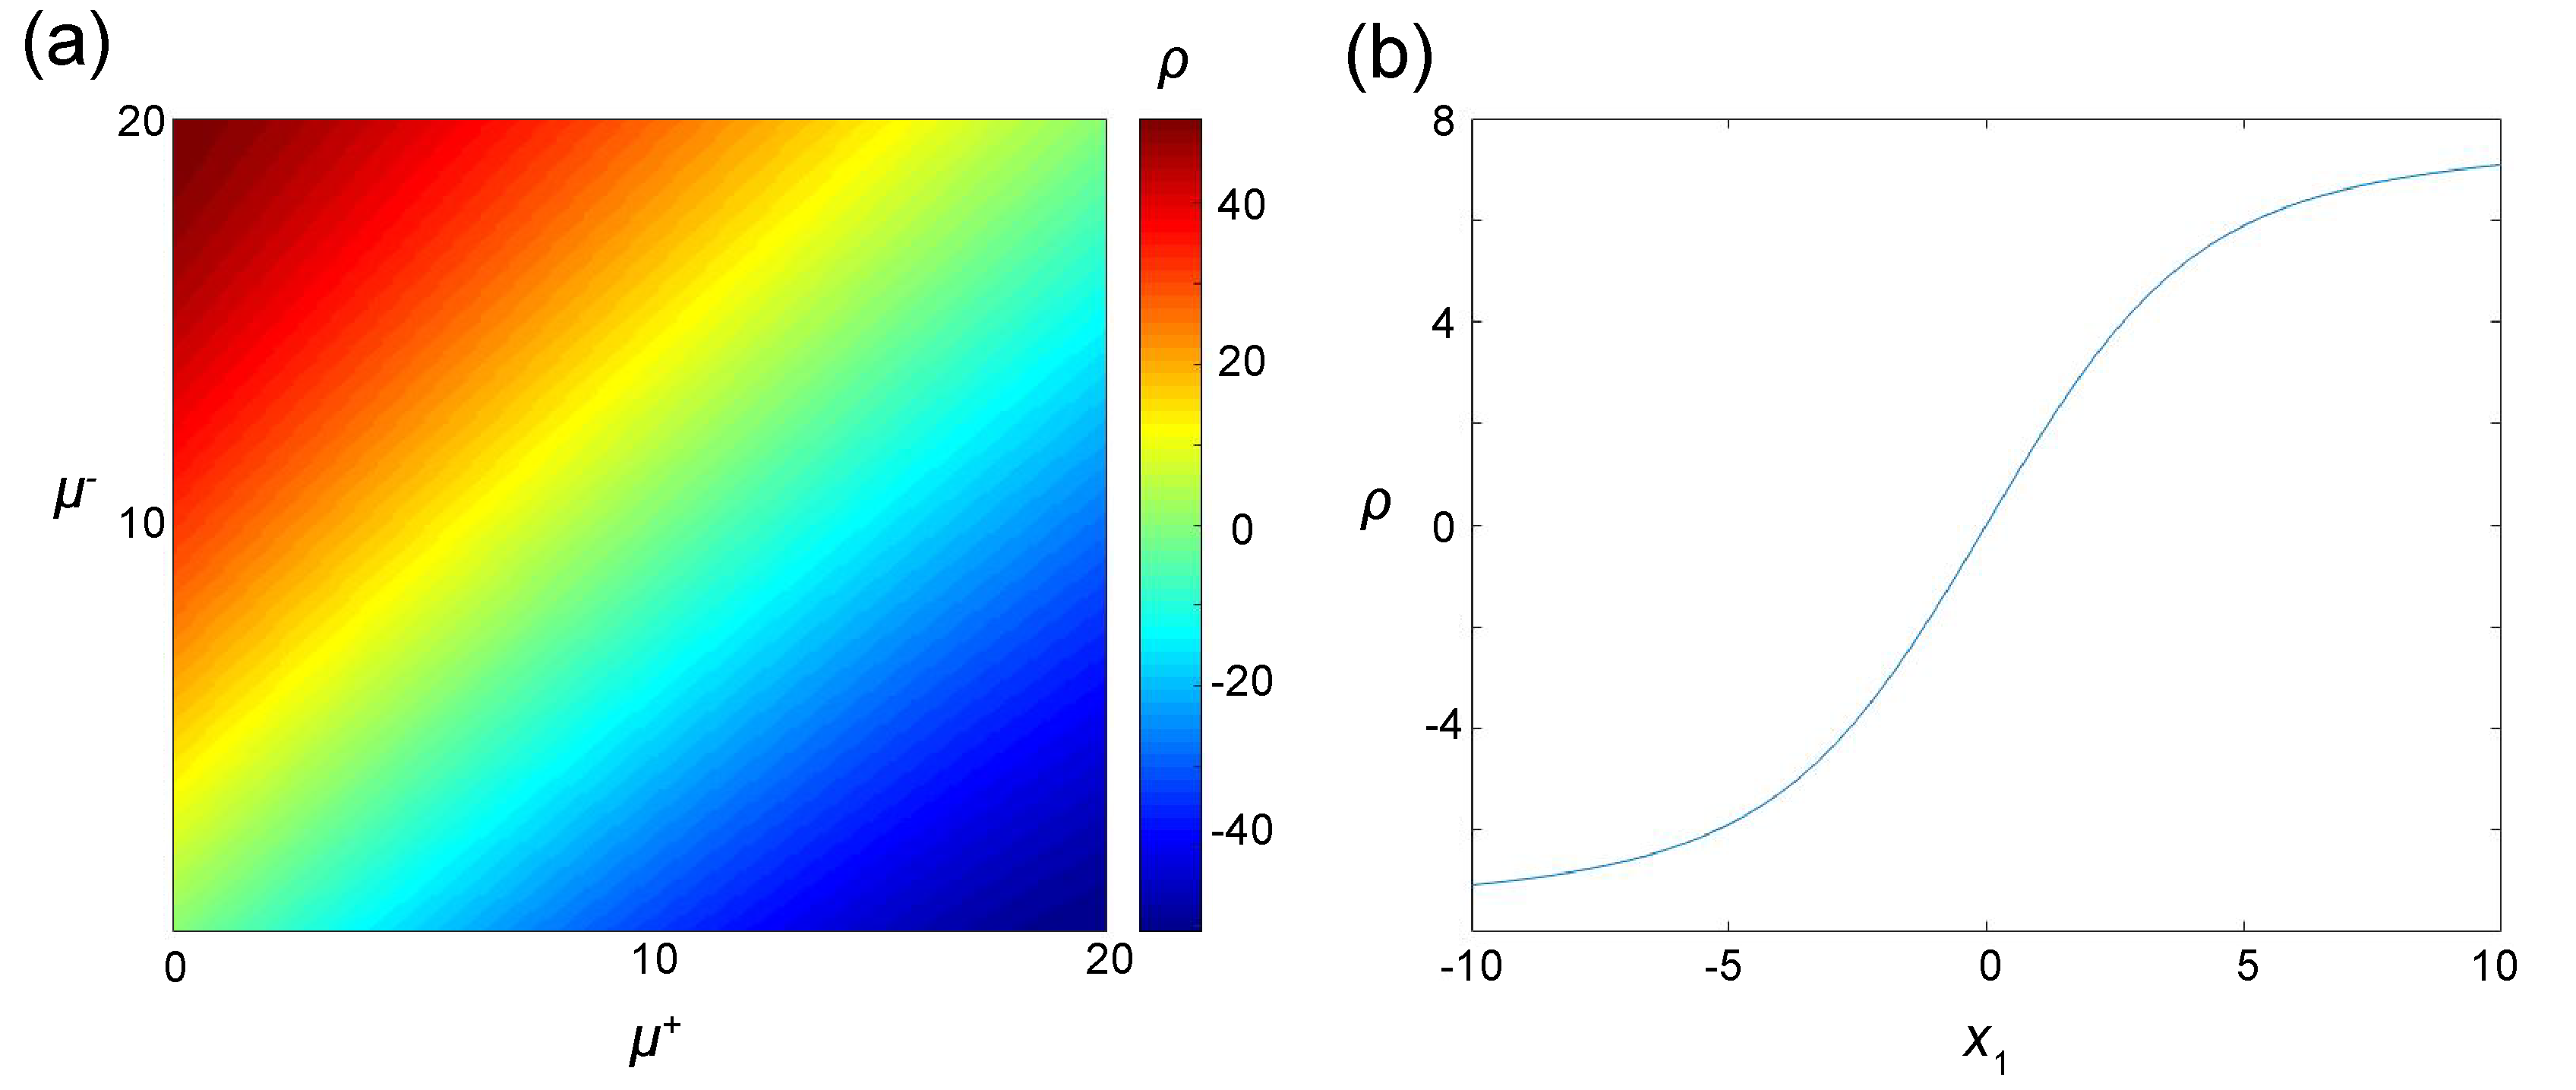
\includegraphics[scale=0.14]{chart/ratefunction.pdf}
			% \caption{\tiny ST经验(净)环流的速率函数图像}
		\end{figure}
		{\tiny (a) 三状态全连接马氏链,$\rho=I_Q(\cdots,\mu^+,\mu^-)-I_Q(\cdots,\mu^-,\mu^+)+(\log\frac{\gamma^+}{\gamma^-})(\mu^+-\mu^-)$的热力图,表明Gallavotti-Cohen 类型涨落定理对ST环流不成立。 \\
		(b) 四状态全连接马氏链,$\rho=I_{\tilde{Q}}(\tilde{\mu}^{c_1},\tilde{\mu}^{c_2},\tilde{\mu}^{c_3})-  I_{\tilde{Q}}(-\tilde{\mu}^{c_1},\tilde{\mu}^{c_2},\tilde{\mu}^{c_3})+(\log\frac{\gamma^{c_1}}{\gamma^{c_1-}})\tilde{\mu}^{c_1}$的函数图像,表明Gallavotti-Cohen 类型涨落定理对ST净环流不成立。}
	\end{block}
\end{frame}

\begin{frame}{环流的涨落定理}{ST环流的涨落定理}
	\begin{block}{一般马氏链ST环流不满足涨落定理}
		\begin{figure}[h]
			\centering
			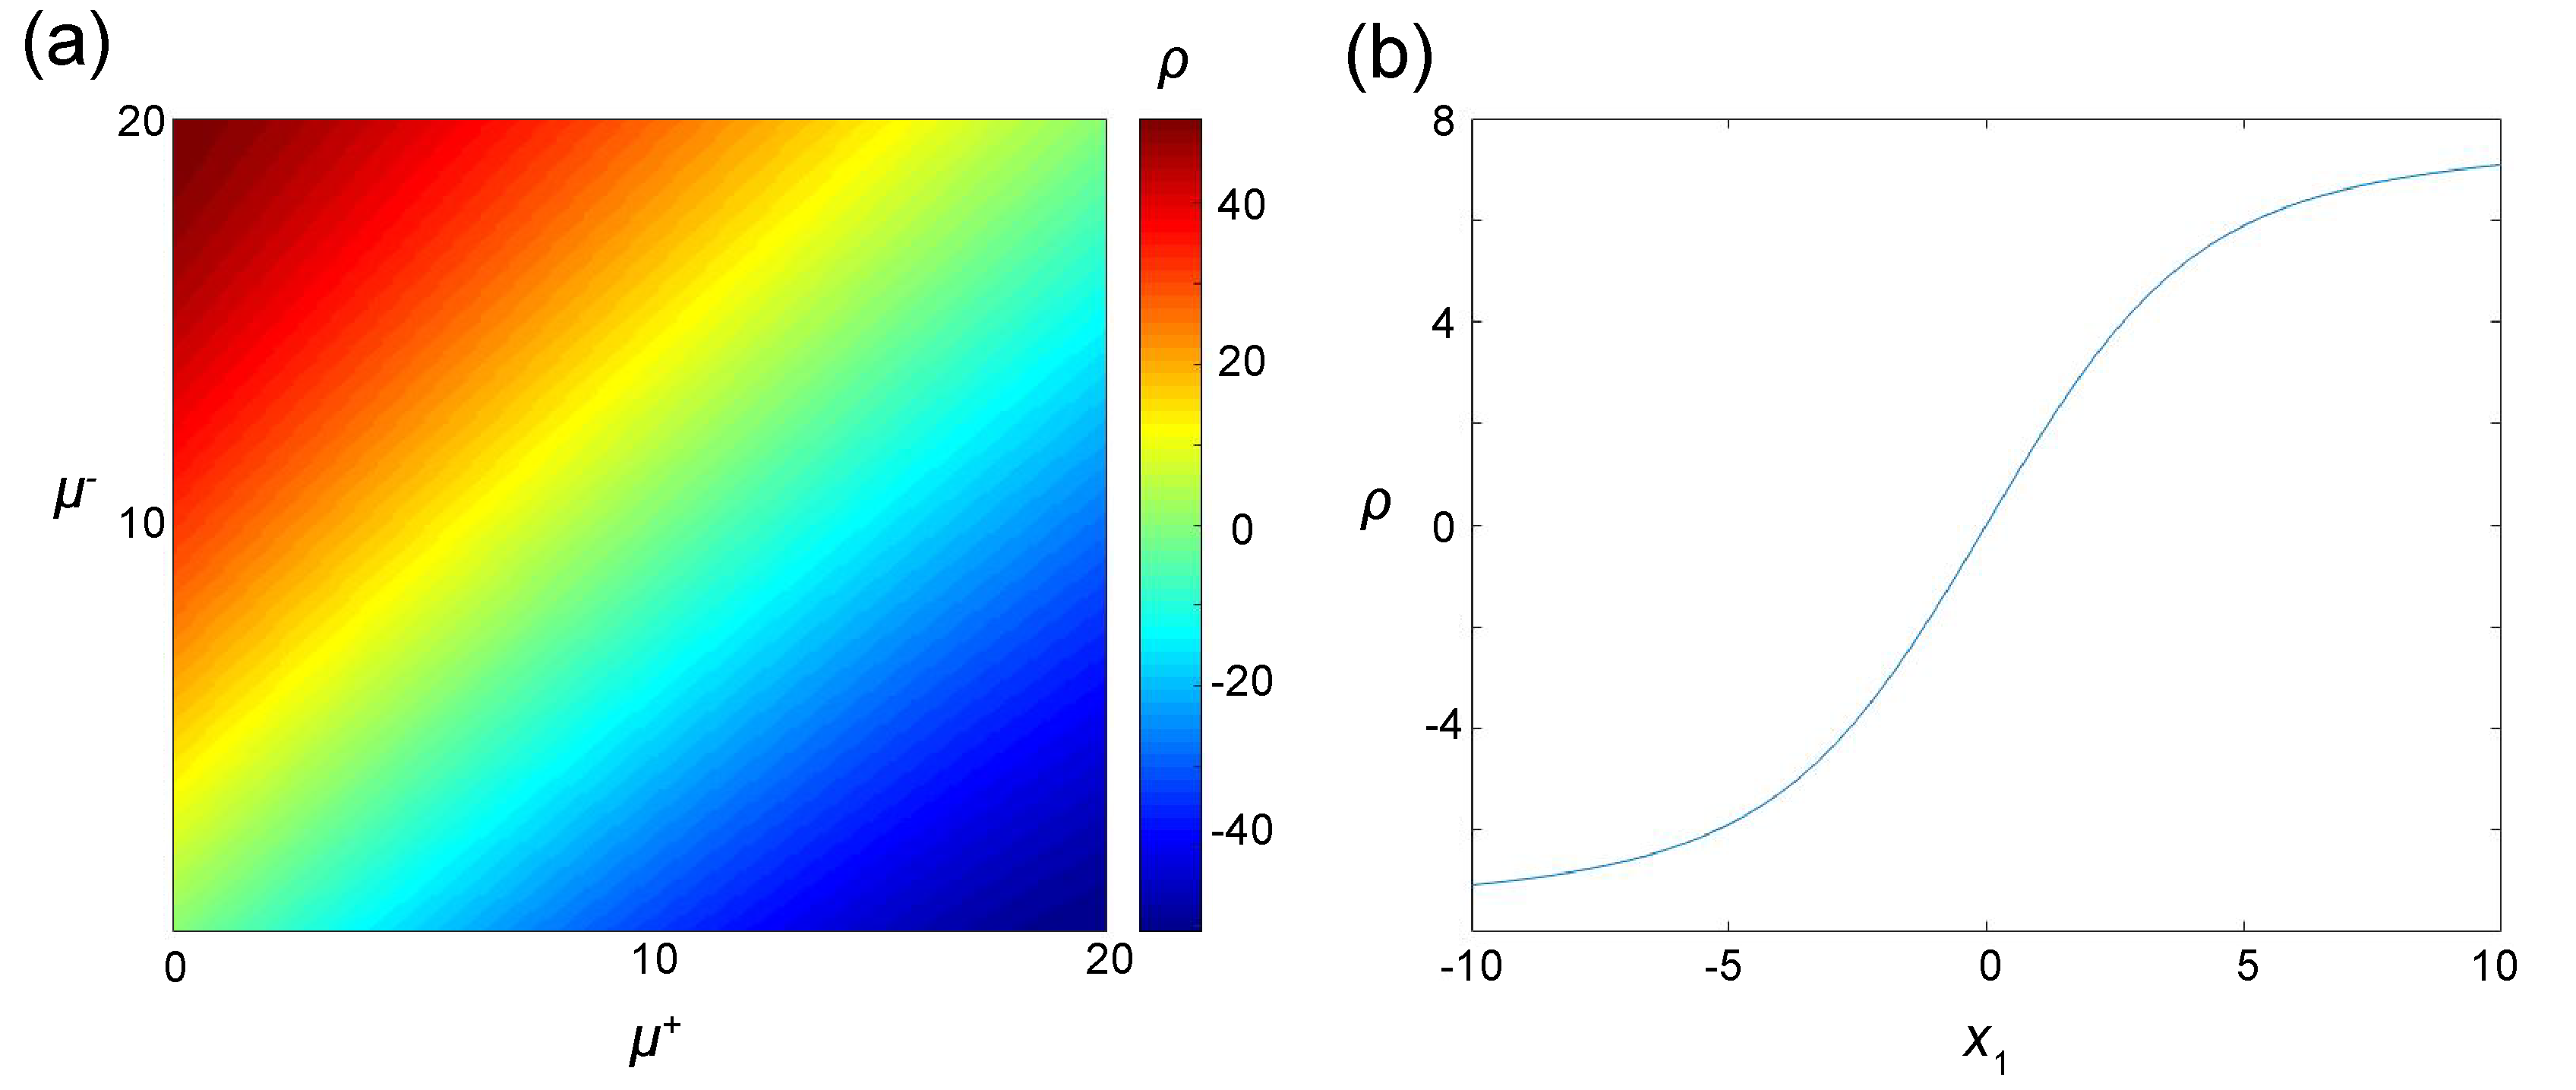
\includegraphics[scale=0.14]{chart/ratefunction.pdf}
			% \caption{\tiny ST经验(净)环流的速率函数图像}
		\end{figure}
		{\tiny 该图(a)说明了 $I_Q(\cdots,\mu^+,\mu^-)$和$I_Q(\cdots,\mu^-,\mu^+)-\log(\gamma^+ /\gamma^-) (\mu^+-\mu^-)$之间的差异,因此有:
		\begin{equation*}
			I_Q(\cdots,\mu^+,\mu^-)
			\neq I_Q(\cdots,\mu^-,\mu^+)-\left(\log\frac{\gamma^+}{\gamma^-}\right)(\mu^+-\mu^-),
		\end{equation*}
		这说明了 Gallavotti-Cohen 类型涨落定理对于ST环流不成立。由于Gallavotti-Cohen 类型涨落定理成立条件最弱,因此其他类型涨落定理也不成立。}
	\end{block}
\end{frame}

\begin{frame}{环流的涨落定理}{ST环流的涨落定理}
	\begin{block}{ST净环流涨落定理}
		周期边界条件下,ST净环流满足暂态涨落定理的弱形式,即:
		\begin{equation*}\label{weak2}
			\begin{split}
				\frac{\Pnum\left(\tilde{Q}^{c_{l_1}}_n=x_1,\cdots, \tilde{Q}^{c_{l_s}}_n=x_{s}\right)}
				{\Pnum\left(\tilde{Q}^{c_{l_1}}_n=-x_1,\cdots, \tilde{Q}^{c_{l_s}}_n=-x_{s}\right)}
				=e^{n\sum_{i=1}^{s}x_i\log\frac{\gamma^{c_{l_i}}}{\gamma^{c_{l_i}-}}}.
			\end{split}
		\end{equation*}
		上图中(b)说明了 $I_{\tilde{Q}}(x_1, x_2, x_3)$ 和 $ I_{\tilde{Q}}(-x_1, x_2, x_3) -\left(\log \gamma^{c_1} / \gamma^{c_1-}\right)\tilde{\mu}^{c_1}$之间的差异,因此:
		\begin{equation*}
			I_{\tilde{Q}}(x_1, x_2, x_3) \neq I_{\tilde{Q}}(-x_1, x_2, x_3) -\left(\log\frac{\gamma^{c_1}}{\gamma^{c_1-}}\right)\tilde{\mu}^{c_1},
		\end{equation*}
		ST经验净环流不满足 Gallavotti-Cohen 类型涨落定理的强形式。
	\end{block}
\end{frame}

\begin{frame}{总结和展望}
	主要工作
	\begin{itemize}
		\item 建立 LE 环流的大偏差原理
		\item 单环马氏链中LE经验环流的速率大偏差函数的表达式
		\item 一般马氏系统的经验ST环流的速率函数的表达式
		\item LE (净)环流是否满足的各种涨落定理
		\item ST (净)环流是否满足的各种涨落定理
	\end{itemize}
	未来展望
	\begin{itemize}
		\item 大偏差速率函数的结果是否可以推广到一般马氏链模型
		\item 除 LE 和ST 环流,其他类型环流是否满足涨落定理
	\end{itemize}
\end{frame}


\begin{frame}
	\begin{center}
		\Huge 谢谢!
	\end{center}
\end{frame}
\end{document}